\chapter{Desarrollo del TFG}
\label{ch:desarrollo}

%\avisoLocalizacionArchivo 

\begin{comment}
En general este capítulo debe describir cómo se ha llegado a la solución del problema incluyendo metodología, planificación y ejecución.

En primer lugar, este capítulo debe tratar con la metodología de trabajo empleada para elaborar el \gls{TFG}.  La metodología puede variar sustancialmente dependiendo del contexto o el área temática en la que se encuadre.  Si es necesario, divide la descripción de la metodología como capítulo independiente.

A continuación, debe describir cómo se ha dividido el problema en una secuencia de fases, tareas o iteraciones y qué cantidad de recursos (tiempo fundamentalmente) se han planificado para cada una.

Por último, debe incluir información sobre la ejecución del proyecto. Cuáles han sido los problemas encontrados y qué desviaciones se han producido en la ejecución.  Dependiendo de la naturaleza del proyecto es posible organizar esta información de manera conjunta con la planificación.
\end{comment}

Este capítulo describe cómo se ha llegado a la solución del problema planteado: La metodología de trabajo empleada, la división del proyecto en fases, y la ejecución real, incluyendo los problemas encontrados y las desviaciones producidas respecto a lo previsto.

De acuerdo con las directrices de integridad y transparencia académica, se hace constar que en el desarrollo y la depuración del código descrito en este capítulo se ha empleado el modelo de lenguaje Claude, de Anthropic, como herramienta de apoyo a la programación. Las decisiones de diseño, la validación de los resultados y su interpretación son responsabilidad del autor.

\section{Metodología de trabajo}
\label{sec:metodologia}

Antes de entrar en los detalles técnicos, este apartado expone la metodología con la que se ha llevado a cabo el proyecto. Se presenta primero el enfoque general ---un desarrollo iterativo e incremental organizado en bloques funcionales---; a continuación, el criterio que ha vertebrado todo el trabajo ---la validación cuantitativa frente a fuentes primarias---; y, por último, las prácticas de ingeniería del software y las herramientas empleadas. Estas tres decisiones responden a un mismo propósito: asegurar que cada resultado descanse sobre una base fiable y trazable antes de construir sobre ella.

\subsection{Enfoque general: desarrollo iterativo e incremental por bloques}

El proyecto se ha abordado siguiendo una metodología iterativa e incremental, organizando el trabajo en bloques funcionales que se construyen y verifican de forma sucesiva. Cada bloque produce un resultado utilizable y validado antes de abordar el siguiente, lo que permite detectar errores de forma temprana y mantener en todo momento una base estable.

Una decisión metodológica central ha sido separar el desarrollo físico del desarrollo de la \gls{IA}, abordando la física en primer lugar. La razón es que la \gls{IA} de maniobras necesita apoyarse en un simulador físico fiable: construir el agente sobre una física no validada haría imposible distinguir si un mal resultado se debe al agente o al simulador.

\subsection{La validación como eje metodológico}
\label{sec:validacion-metodo}

El criterio que ha guiado todo el trabajo físico es la validación cuantitativa contra fuentes primarias. Ningún dato numérico relevante se ha dado por bueno sin contrastarlo con una fuente trazable: librerías de referencia oficiales, conjuntos de datos in-situ de misiones espaciales (archivo \gls{NASA}-\gls{PDS}) o artículos científicos revisados por pares.

Esta filosofía se reforzó tras una experiencia concreta: al contrastar unos valores de densidad de la atmósfera de Júpiter proporcionados por una \gls{IA} generalista con los datos reales de la sonda Galileo, se detectó un error de hasta un factor $2500$. A raíz de ello se adoptó como regla del proyecto no emplear datos numéricos procedentes de IAs generalistas sin verificación. Este principio de trazabilidad y honestidad metodológica se considera uno de los aportes del trabajo.

\subsection{Prácticas de ingeniería del software y herramientas}

Para asegurar la calidad y la mantenibilidad del código se han seguido varias prácticas: la refactorización del código inicial (scripts monolíticos) hacia un módulo unificado y reutilizable; una batería de pruebas automáticas de verificación que recorre los nueve cuerpos; y una
documentación trazable en la que cada cuerpo dispone de un informe con sus fuentes científicas.

El desarrollo se ha realizado en Python~3.10.11 sobre Windows~11, con el entorno de desarrollo PyCharm y un entorno virtual aislado (\texttt{venv}). Las bibliotecas principales empleadas, con su versión y su función, se recogen en la Tabla~\ref{tab:herramientas}.

\begin{table}[htbp]
  \centering
  \caption{Bibliotecas principales empleadas en el desarrollo, con su versión y su función.}
  \label{tab:herramientas}
  \begin{tabular}{l c p{6.6cm}}
    \hline
    \textbf{Biblioteca} & \textbf{Versión} & \textbf{Función} \\
    \hline
    \texttt{poliastro}~\cite{poliastro}             & 0.17.0 & Mecánica orbital y propagación \\
    \texttt{astropy}~\cite{astropy2022}             & 5.3.4  & Base de \texttt{poliastro} (constantes, tiempos y unidades) \\
    \texttt{NumPy}~\cite{numpy}                     & 1.26.4 & Cálculo numérico \\
    \texttt{SciPy}~\cite{scipy}                     & 1.15.3 & Cálculo numérico \\
    \texttt{Matplotlib}~\cite{matplotlib}           & 3.7.3  & Visualización 2D \\
    \texttt{Plotly}                                 & 5.24.1 & Visualización 3D interactiva \\
    \texttt{ussa1976}~\cite{ussa1976}               & 0.3.4  & Modelo de atmósfera estándar terrestre (USSA-76) \\
    \texttt{Gymnasium}~\cite{gymnasium}             & 1.2.3  & Definición de los entornos de \gls{RL} \\
    \texttt{stable-baselines3}~\cite{raffin2021sb3} & 2.8.0  & Algoritmo \gls{PPO} \\
    \texttt{PyTorch}~\cite{pytorch}& 2.12.0 & Redes neuronales \\
    \texttt{openai} (SDK)      & 2.44.0 & Cliente de la capa \gls{LLM}, conectada al modelo Llama~3.3 servido por Groq \\
    \hline
  \end{tabular}
\end{table}

\section{Desarrollo e implementación de la física}
\label{sec:implementacion}

Esta sección describe las partes principales del sistema físico y su funcionamiento, incluyendo la formulación en la que se sustentan (los conceptos de mecánica orbital empleados se introdujeron en el Capítulo~\ref{ch:fundamentos}). El desarrollo de los agentes de inteligencia artificial, que se apoyan en esta base física, se trata aparte en la Sección~\ref{sec:ia}.

\subsection{Organización del software}
\label{sec:scripts}

El sistema se ha estructurado en \textbf{módulos funcionales}, cada uno responsable de una parte bien delimitada del problema. A continuación se describen, indicando entre paréntesis el archivo o carpeta que los implementa:

\begin{itemize}
  \item \textbf{Módulo atmosférico}
        (\texttt{Densidades\_atmosferica\_optimizado.py}): contiene la clase \texttt{Planeta} y el modelo atmosférico por capas de los nueve cuerpos, junto con el simulador de decaimiento orbital basado en energía (Bloque~0). Es la base reutilizable por el resto del sistema.
  \item \textbf{Módulo de propagación orbital}
        (\texttt{Pruebas\_perturbaciones\_optimizado.py}): propagador tridimensional con perturbación $J_2$ y arrastre atmosférico, construido sobre el propagador de Cowell de \texttt{poliastro} (Bloque~2).
  \item \textbf{Módulo de maniobras} (\texttt{Orbitas\_en\_planetas.py},
        \texttt{Orbitas\_entre\_planetas.py}): impulsos, transferencias de Hohmann, problema de Lambert y diagramas \textit{porkchop}, que son la base de las maniobras clásicas que emplea la inteligencia artificial.
  \item \textbf{Módulo de agentes de \gls{RL}} (\texttt{ia/}): los cinco agentes que aprenden las maniobras ---transferencias impulsivas, cambio de plano, aerofrenado y mantenimiento orbital---, cada uno con su entorno, entrenamiento y evaluación (\texttt{env\_*}, \texttt{train\_*}, \texttt{evaluar\_*}), junto con los óptimos clásicos que actúan de juez (\texttt{baselines.py}). Se apoya en los módulos físicos anteriores, sobre los que los agentes practican.
  \item \textbf{Módulo de orquestación en lenguaje natural} (\texttt{ia/llm\_*.py}): la capa basada en un \gls{LLM} que interpreta las peticiones del usuario, invoca la herramienta adecuada ---un agente o un solucionador clásico--- mediante \textit{tool use} y explica los resultados obtenidos. Reúne el orquestador, las herramientas de cálculo y las de dibujo.
  \item \textbf{Módulo de validación} (\texttt{datos\_validacion/}, \texttt{tests/}): contraste del modelo frente a datos de misiones reales y reconstrucciones, junto con la batería de pruebas automáticas del propagador.
  \item \textbf{Módulo de visualización} (transversal, basado en \texttt{Plotly} y \texttt{Matplotlib}): representación tridimensional interactiva de las órbitas y gráficas bidimensionales comparativas (órbita ideal frente a realista), utilizadas por los módulos anteriores.
\end{itemize}

\begin{figure}[!htbp]
  \centering
  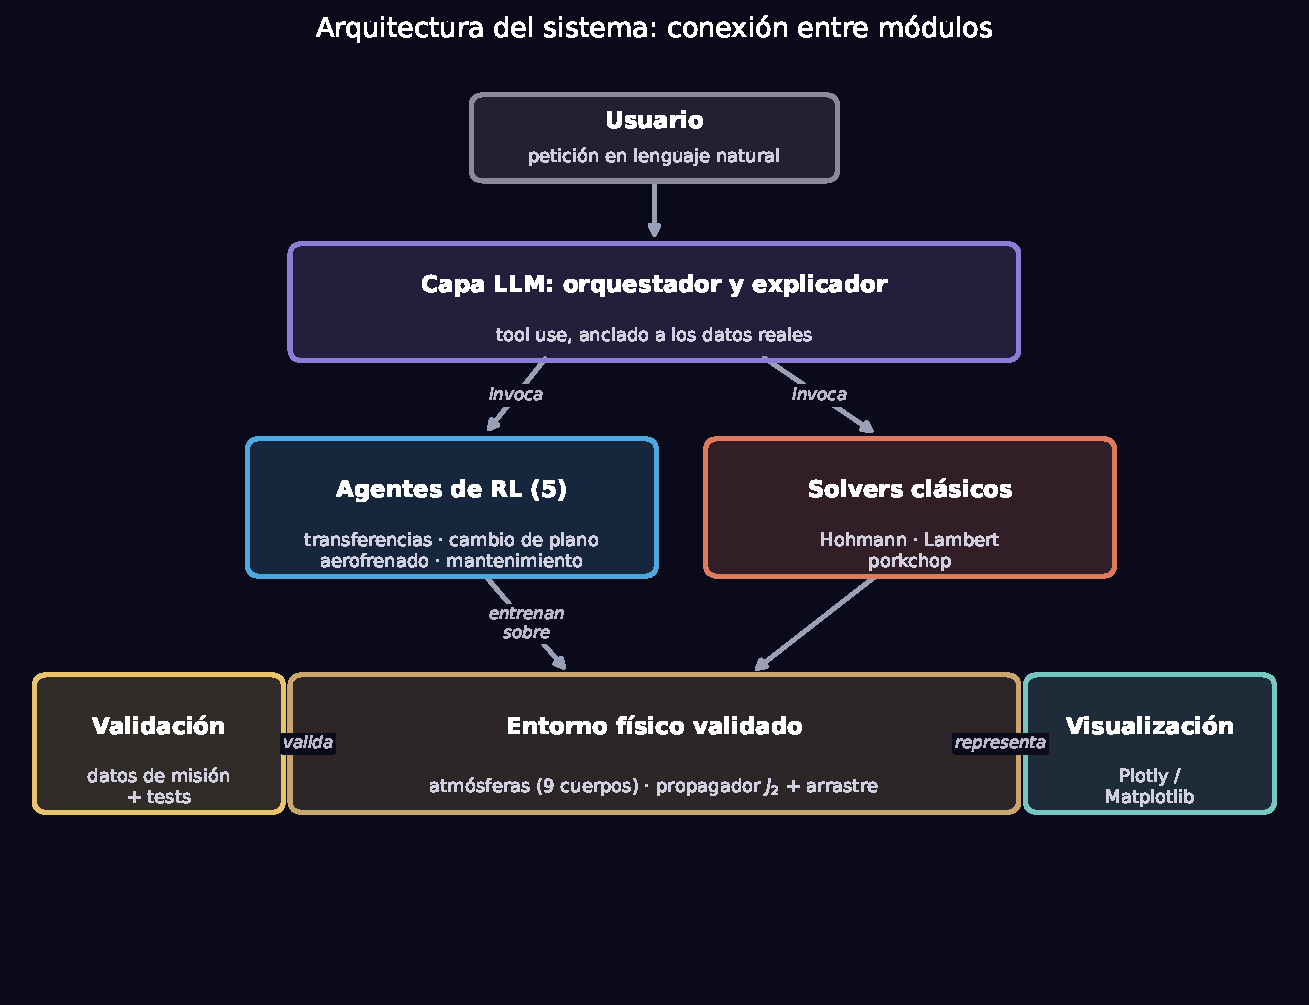
\includegraphics[width=0.9\textwidth]{tex/imagenes/arquitectura_modulos.pdf}
  \caption{Arquitectura del sistema y conexión entre módulos. Elaboración propia.}
  \label{fig:arquitectura}
\end{figure}

La Figura~\ref{fig:arquitectura} resume cómo se conectan estos módulos: el usuario plantea la maniobra en lenguaje natural, la capa \gls{LLM} interpreta la petición e invoca el agente o el solucionador más adecuado, y estos actúan sobre el entorno físico validado. La validación y la visualización operan de forma transversal sobre todo el conjunto.

\subsection{Modelo atmosférico: del equilibrio hidrostático al perfil exponencial}
\label{sec:hidrostatica}

La densidad de la atmósfera de cada cuerpo se modela mediante un perfil \textit{piecewise}-exponencial. Su forma no es arbitraria, sino que se deduce de dos principios físicos.

En primer lugar, el equilibrio hidrostático establece que la variación de presión con la altura compensa el peso de la columna de gas (Ecuación \ref{eq:hidrostatica}):

\begin{equation}
  \frac{dP}{dh} = -\rho\, g .
  \label{eq:hidrostatica}
\end{equation}

En segundo lugar, la ley de los gases ideales relaciona presión y densidad a través de la temperatura $T$ y el peso molecular medio $\bar{M}$ (Ecuación \ref{eq:gas-ideal}):
\begin{equation}
  P = \frac{\rho}{\bar{M}} R_g\, T
  \qquad\Longrightarrow\qquad
  \rho = \frac{P\,\bar{M}}{R_g\,T},
  \label{eq:gas-ideal}
\end{equation}
con $R_g = 8{,}314\ \mathrm{J\,mol^{-1}\,K^{-1}}$ la constante de los gases.

Sustituyendo \eqref{eq:gas-ideal} en \eqref{eq:hidrostatica} se obtiene una ecuación diferencial separable (Ecuación \ref{eq:escala}):
\begin{equation}
  \frac{dP}{P} = -\frac{\bar{M} g}{R_g\,T}\, dh = -\frac{dh}{H},
  \qquad\text{donde}\qquad
  H \equiv \frac{R_g\,T}{\bar{M}\, g}.
  \label{eq:escala}
\end{equation}
La magnitud $H$ es la altura de escala: la altura en la que la densidad disminuye en un factor $e$. Depende de la temperatura, del peso molecular y de la gravedad, lo que explica que las atmósferas calientes, de gas ligero y gravedad baja (gigantes gaseosos) sean mucho más extensas que la terrestre.

Integrando la Ecuación \ref{eq:escala} dentro de una capa en la que $T$, $\bar{M}$ y $g$ se suponen aproximadamente constantes (hipótesis isoterma por tramos), desde el límite inferior $h_{\min}$ de la capa, resulta el perfil empleado en el modelo (Ecuación \ref{eq:perfil}):

\begin{equation}
  \;\rho(h) = \rho_{\text{base}}\,
  \exp\!\left(-\frac{h - h_{\min}}{H}\right)\;
  \label{eq:perfil}
\end{equation}

La atmósfera de cada cuerpo se divide en $N$ capas y se aprecian los perfiles de densidad en los diferentes planetas en la Figura~\ref{fig:perfil-densidad}. Las densidades de referencia $\rho_{\text{base}}$ de cada capa son las observaciones (procedentes de las fuentes validadas); las alturas de escala $H_i$ no se introducen a mano, sino que se derivan para garantizar la continuidad del perfil en las fronteras entre capas (Ecuación \ref{eq:continuidad}):
\begin{equation}
  H_i = \frac{h_{\min,\,i-1} - h_{\min,\,i}}      {\ln\!\left(\rho_{\text{base},\,i}\,/\,\rho_{\text{base},\,i-1}\right)} .
  \label{eq:continuidad}
\end{equation}
Esta condición tiene además un valor de auto-comprobación: si la $H$ derivada por la Ecuación \eqref{eq:continuidad} se aleja mucho de la altura de escala física $R_g T/(\bar{M} g)$, es señal de que alguna densidad de referencia es incorrecta. Este mecanismo permitió detectar un error de calibración en Neptuno.

\begin{figure}[htbp]
  \centering
  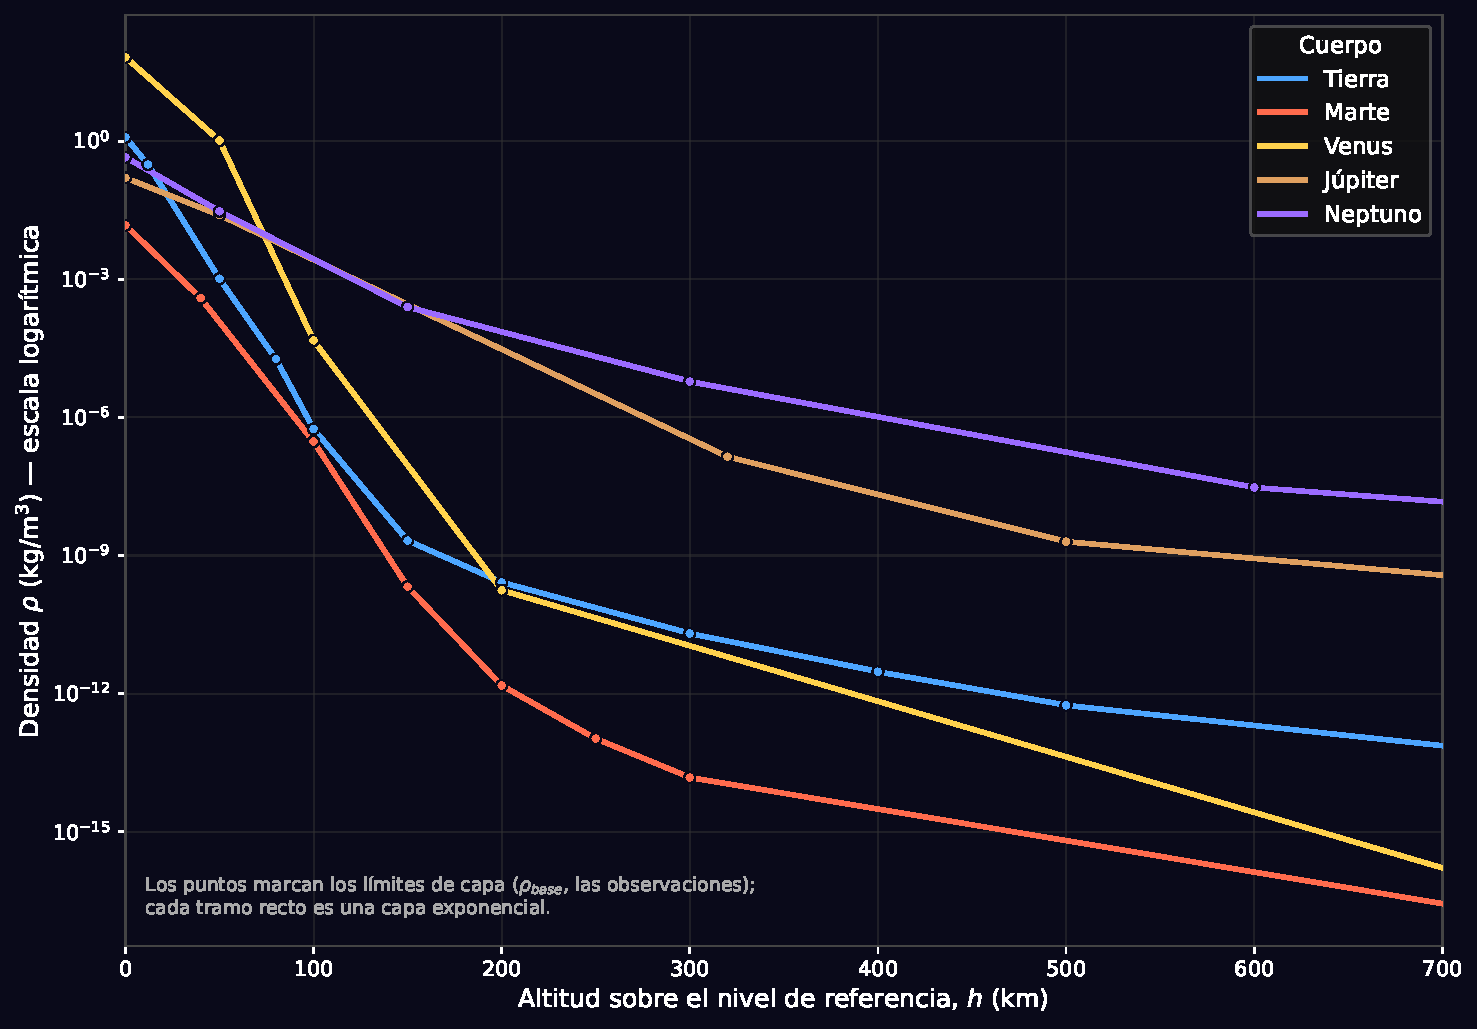
\includegraphics[width=0.85\textwidth]{tex/imagenes/fig_perfil_densidad.pdf}
  \caption{Perfil de densidad $\rho(h)$ del modelo de capas para cinco cuerpos. Elaboración propia.}
  \label{fig:perfil-densidad}
\end{figure}


\subsection{Modelo de decaimiento orbital por energía}
\label{sec:decaimiento}

El primer simulador calcula el decaimiento de la órbita por arrastre mediante un balance de energía, bajo la hipótesis de órbita cuasi-circular en cada instante (válida cuando el arrastre es una perturbación pequeña). La energía orbital y la velocidad circular a distancia $r$ del centro son respectivamente (Ecuación \ref{eq:energia}):
\begin{equation}
  E = -\frac{G M m}{2\,r},
  \qquad
  v = \sqrt{\frac{G M}{r}} .
  \label{eq:energia}
\end{equation}

La fuerza de arrastre y la potencia que disipa (energía perdida por unidad de tiempo) son (Ecuación \ref{eq:potencia}):
\begin{equation}
  F_{\text{drag}} = \tfrac{1}{2}\,\rho(h)\, v^{2}\, C_d\, A,
  \qquad
  \frac{dE}{dt} = -F_{\text{drag}}\, v ,
  \label{eq:potencia}
\end{equation}
donde $C_d$ es el coeficiente de arrastre y $A$ el área frontal del satélite. En cada paso temporal $dt$ se actualiza la energía y se recupera el nuevo radio despejando de \eqref{eq:energia}, obteniendo la Ecuación \ref{eq:actualizacion}:
\begin{equation}
  E_{n+1} = E_{n} - F_{\text{drag}}\, v\, dt,
  \qquad
  r_{n+1} = -\frac{G M m}{2\,E_{n+1}},
  \qquad
  h_{n+1} = r_{n+1} - R .
  \label{eq:actualizacion}
\end{equation}

El paso temporal es adaptativo: se reduce a la mitad si en un paso se
disiparía más del $0,1\%$ de la energía, si la órbita pasara a ser abierta o si la caída de radio superase un umbral. Así se mantiene la precisión en las capas densas sin penalizar el cómputo en las altas.

\subsection{El término \texorpdfstring{$J_2$}{J2}: el achatamiento planetario}
\label{sec:j2}

Hasta aquí, la gravedad se ha modelado asumiendo el planeta como una masa puntual ($-\mu/r$), lo que genera órbitas elípticas cerradas e inmutables (órbitas keplerianas). Sin embargo, los planetas reales no son esferas perfectas: su rotación introduce un achatamiento que genera un abultamiento de masa en la zona ecuatorial. Este exceso de masa rompe la simetría esférica del campo gravitatorio, introduciendo perturbaciones en la órbita del satélite.

El coeficiente $J_2$ corresponde a una perturbación conservativa y representa el primer término ---y el dominante--- del desarrollo del potencial gravitatorio en armónicos zonales\footnote{Un desarrollo en armónicos esféricos expresa el campo gravitatorio de un cuerpo no esférico como una suma de términos de detalle creciente, de forma análoga a cómo un sonido se descompone en sus armónicos. Los términos zonales (coeficientes $J_2, J_3, J_4, \dots$) son los que dependen únicamente de la latitud, y describen las desviaciones del campo simétricas respecto al eje de rotación del planeta, como el abultamiento ecuatorial.} (Ecuación \ref{eq:potencial-j2}):
\begin{equation}
  U(r, \phi) = -\frac{\mu}{r} \left[ 1 - J_2 \left(\frac{R}{r}\right)^{2}
  \frac{3\sin^{2}\phi - 1}{2} \right] ,
  \label{eq:potencial-j2}
\end{equation}
donde $R$ es el radio ecuatorial del cuerpo central y $\phi$ la latitud planetaria. El coeficiente $J_2$ es adimensional y cuantifica la desviación geométrica respecto a la esfera perfecta. En la Tierra su valor es de aproximadamente $1{,}08\times10^{-3}$, mientras que en los gigantes gaseosos es un orden de magnitud mayor, debido a su rápida rotación y menor densidad (por ejemplo, $\approx 1{,}47\times10^{-2}$ en Júpiter).\footnote{Los coeficientes $J_2$ empleados se toman de \texttt{poliastro.bodies} ---y, para la Luna y Mercurio, se fijan a mano---, con respaldo en las fuentes primarias de los respectivos campos gravitatorios: \cite{iers2010} para la Tierra, \cite{caltechGE131} para los planetas, \cite{jupiterGravity2019} para Júpiter, \cite{iess2019saturn} para Saturno, \cite{jacobson2014} para Urano, \cite{zuber2013} para la Luna y \cite{mazarico2014} para Mercurio.}

Físicamente, el abultamiento ecuatorial ejerce sobre el satélite una fuerza gravitatoria adicional que no apunta hacia el centro de masas del planeta. Esto genera un torque neto sobre el plano orbital y, como consecuencia, el momento angular de la órbita reacciona precesando, se explica con la Figura~\ref{fig:torque-j2}. Ello altera los elementos orbitales de dos formas diferenciadas:
\begin{itemize}
  \item \textbf{Efectos periódicos:} oscilaciones a corto plazo (dentro de cada revolución) en el semieje mayor ($a$), la excentricidad ($e$) y la inclinación ($i$), cuyo promedio a largo plazo es nulo.
  \item \textbf{Efectos seculares:} un cambio acumulativo y continuo en la orientación de la órbita; en concreto, la regresión nodal (giro continuo del plano orbital, medido a través del \gls{RAAN}, $\Omega$) y la precesión del perigeo (giro del argumento del perigeo, $\omega$).
\end{itemize}

\begin{figure}[htbp]
  \centering
  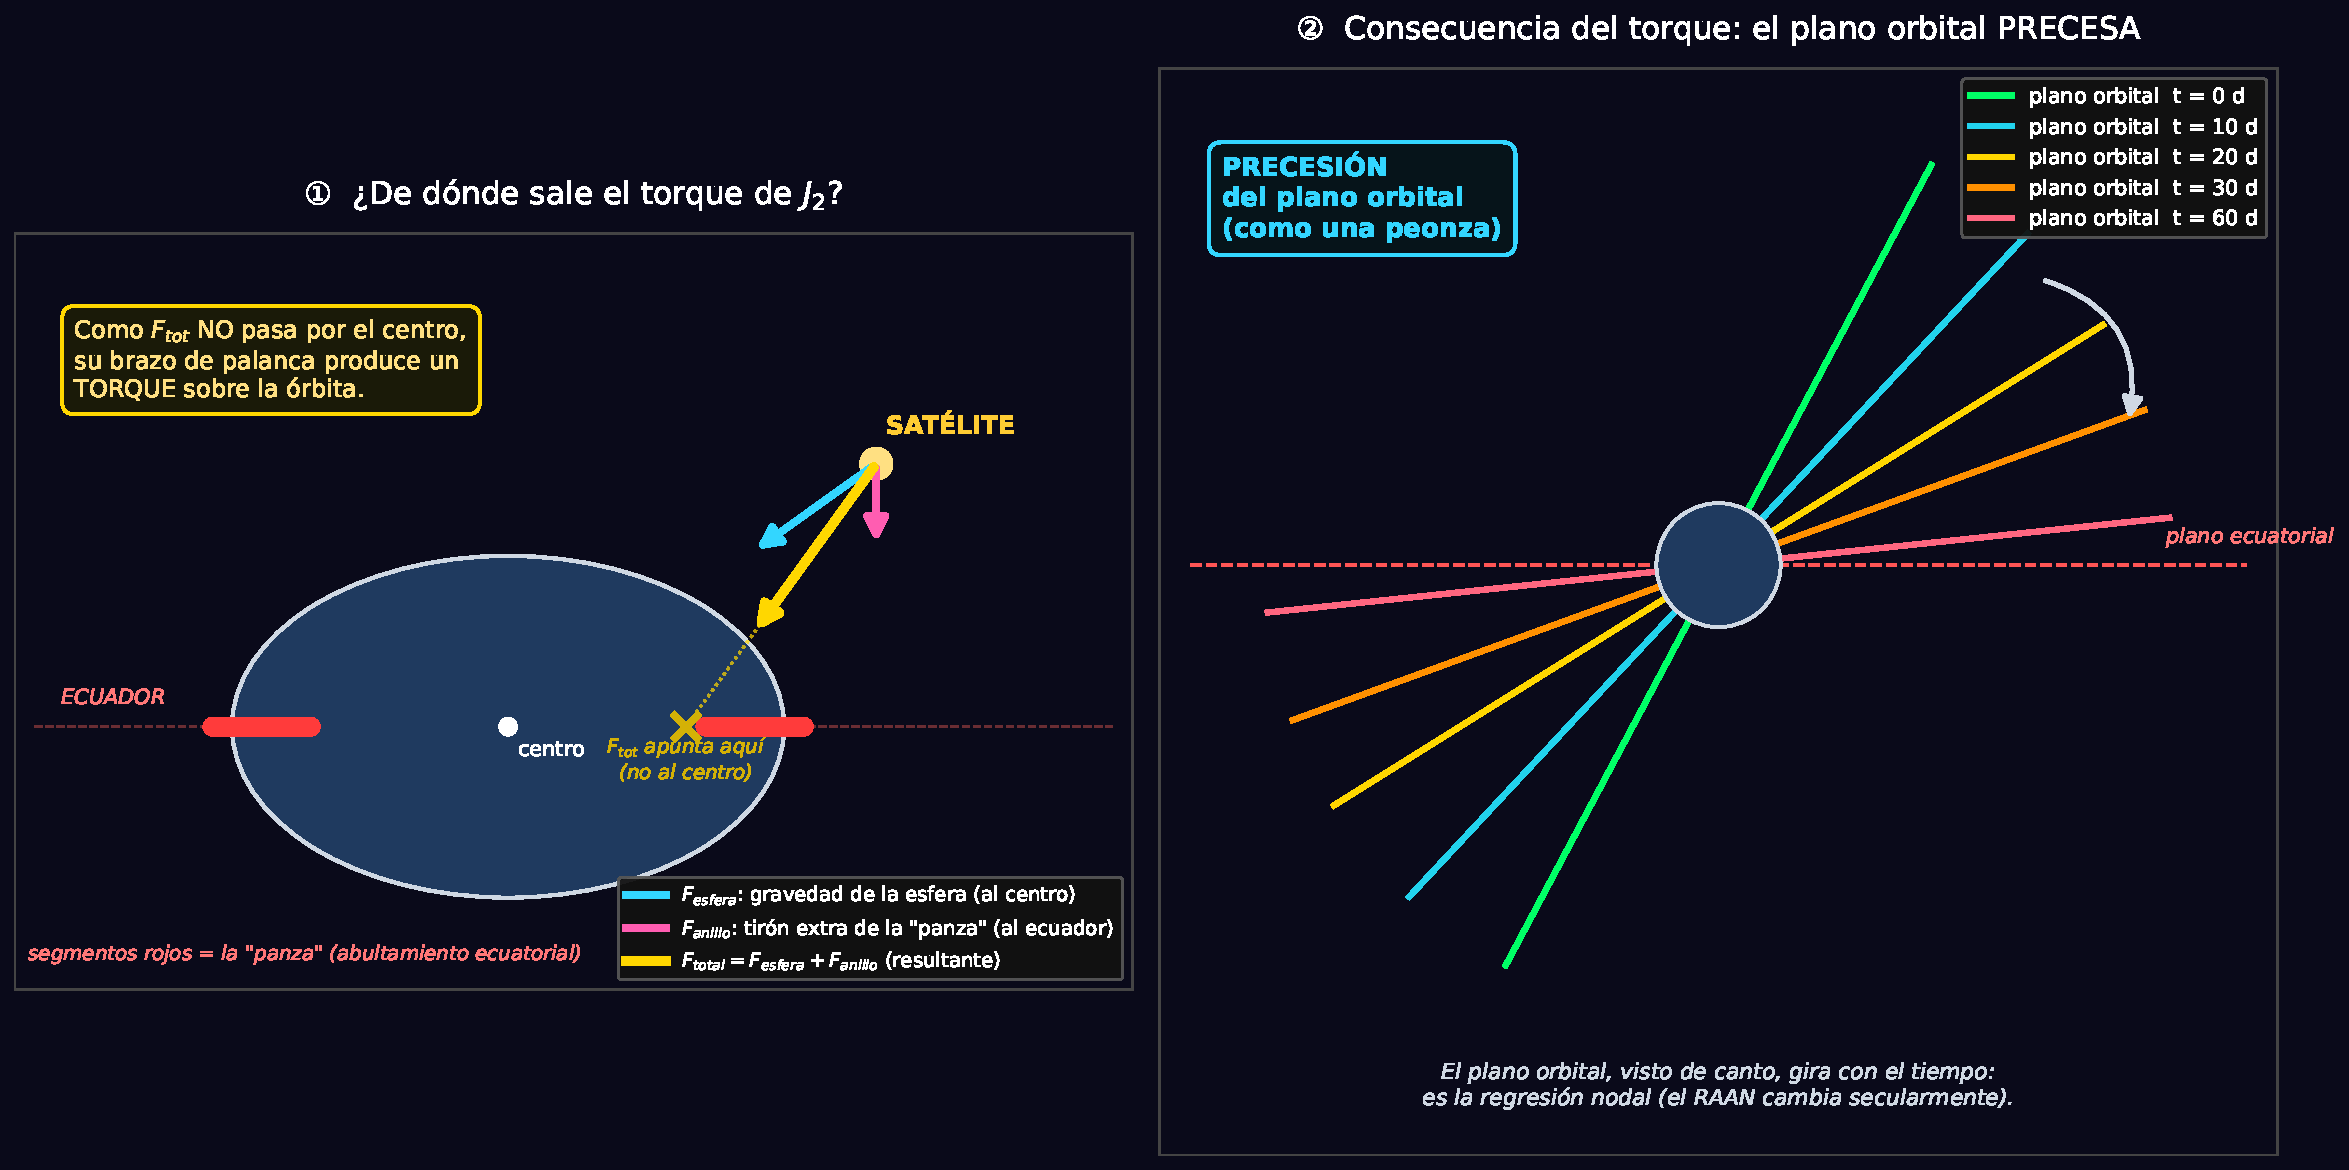
\includegraphics[width=\textwidth]{tex/imagenes/fig_torque_j2.pdf}
  \caption{Origen físico de la perturbación $J_2$ y su efecto secular. Elaboración propia.}
  \label{fig:torque-j2}
\end{figure}

La tasa de regresión nodal acumulada se empleará posteriormente para validar el propagador desarrollado (Sección~\ref{sec:brouwer}). En la implementación numérica, la aceleración perturbativa $\vec{a}_{J_2}$ se obtiene como el gradiente del término de $J_2$ de la Ecuación \ref{eq:potencial-j2}, calculada de forma eficiente mediante la rutina \texttt{J2\_perturbation} de la librería \texttt{poliastro}.

\subsection{Propagación orbital con perturbaciones: el método de Cowell}
\label{sec:propagador}

El modelo de energía (Sección~\ref{sec:decaimiento}) describe bien el decaimiento medio, pero asume órbita circular y no captura la geometría tridimensional ni el efecto del achatamiento. 

La técnica empleada es el método de Cowell, que consiste en integrar numéricamente la ecuación del movimiento completa, sumando en cada instante la gravedad central y todas las perturbaciones, en lugar de usar la solución analítica de Kepler (válida únicamente para el problema de dos cuerpos sin perturbar). La ecuación que se integra es (Ecuación \ref{eq:movimiento}):
\begin{equation}
  \ddot{\vec{r}} = -\frac{\mu}{r^{3}}\,\vec{r}
  \;+\; \vec{a}_{J_2}
  \;+\; \vec{a}_{\text{drag}} ,
  \label{eq:movimiento}
\end{equation}
esto es: aceleración total $=$ gravedad central $+$ achatamiento $+$ arrastre. El primer término es la atracción kepleriana hacia el centro del planeta; $\vec{a}_{J_2}$ es la perturbación por achatamiento (Sección~\ref{sec:j2}); y $\vec{a}_{\text{drag}}$ es el frenado atmosférico. La integración la realiza el \texttt{CowellPropagator} de \texttt{poliastro}.

El término de arrastre se calcula con el modelo de capas propio y, de forma realista, con la atmósfera en rotación solidaria con el planeta (Ecuación \ref{eq:drag-vec}):
\begin{equation}
  \vec{a}_{\text{drag}} = -\tfrac{1}{2}\,\rho(h)\, C_d \,\frac{A}{m}\,
  |\vec{v}_{\text{rel}}|\;\vec{v}_{\text{rel}},
  \qquad
  \vec{v}_{\text{rel}} = \vec{v} - \vec{\omega}\times\vec{r} .
  \label{eq:drag-vec}
\end{equation}
La clave está en $\vec{v}_{\text{rel}}$: el arrastre depende de la velocidad del satélite respecto al aire, no respecto a un sistema fijo. Como la atmósfera gira solidaria con el planeta, su velocidad local es $\vec{\omega}\times\vec{r}$ (con $\vec{\omega}$ la velocidad angular de rotación) y se resta a la del satélite. La densidad $\rho(h)$ procede del modelo atmosférico de la Sección~\ref{sec:hidrostatica}.

Para extraer el decaimiento secular (la pérdida real de altitud por
arrastre) sin contaminarlo con las oscilaciones periódicas que induce $J_2$, se ajusta una recta a la altitud sobre la segunda mitad de la trayectoria: así se evita el transitorio inicial y el ajuste lineal promedia el bamboleo.

En la Figura~\ref{fig:efectos-j2drag} se pueden ver cómo varían ciertos parámetros de la orbita cuando se combina el drag con J2. Comentándolos de arriba a abajo, el panel \textbf{(1)} muestra la altitud instantánea, el $J_2$ produce el dentado periódico y el arrastre el descenso secular, que se mide con un ajuste lineal sobre la segunda mitad de la trayectoria (pendiente $-0{,}1435$ km/día; en verde, la órbita ideal kepleriana, constante). El panel \textbf{(2)} muestra el apogeo y perigeo, el $J_2$ los separa (induce excentricidad) mientras el arrastre baja ambos. El panel \textbf{(3)} muestra la excentricidad, parte de cero (órbita circular) y el $J_2$ la induce hasta $\sim 0{,}0017$ y el panel \textbf{(4)} muestra la regresión nodal, el plano orbital precesa, con $\Delta\Omega = -149{,}3^\circ$ en la simulación frente a $-148{,}5^\circ$ de la fórmula de Brouwer.

\begin{figure}[htbp]
  \centering
  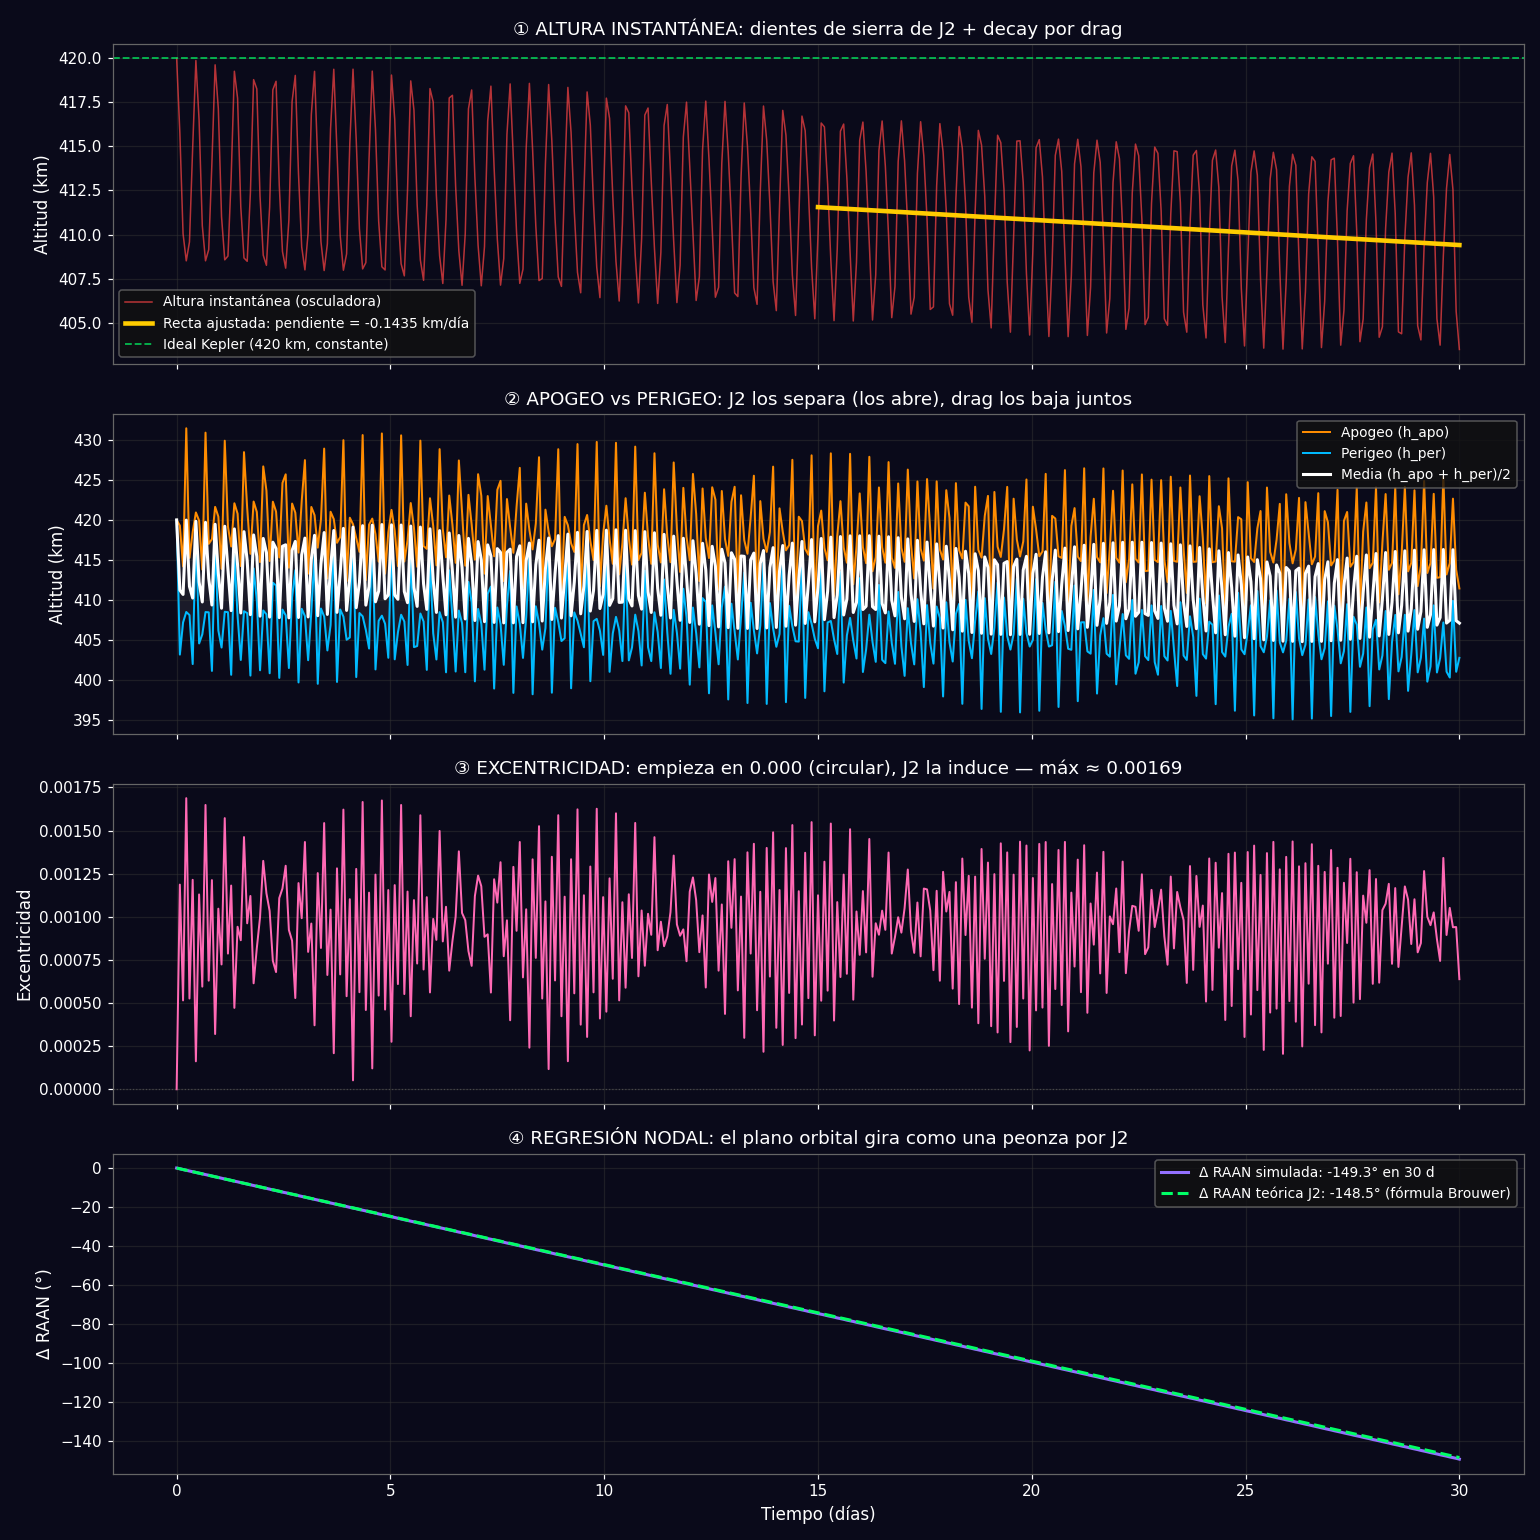
\includegraphics[width=\textwidth]{tex/imagenes/efectos_J2_drag.png}
  \caption{Efectos combinados de $J_2$ y arrastre sobre una órbita de la \gls{ISS} (420 km, 30 días). Elaboración propia}
  \label{fig:efectos-j2drag}
\end{figure}

\subsection{Verificación del propagador: regresión nodal frente a Brouwer}
\label{sec:brouwer}
Para comprobar que el propagador implementa correctamente el efecto de $J_2$, se ha contrastado la regresión nodal simulada (el giro del plano orbital, medido a través de la deriva de la ascensión recta del nodo ascendente, $\Omega$; véase la Sección \ref{sec:elementos}) con la predicción analítica clásica. La teoría de satélites artificiales de Brouwer~(1959)~\cite{brouwer1959} proporciona, a primer orden, la tasa de regresión nodal secular (Ecuación \ref{eq:brouwer}):
\begin{equation}
  \frac{d\Omega}{dt} = -\frac{3}{2}\,J_2\, n \left(\frac{R}{p}\right)^{2}\cos i ,
  \qquad n = \sqrt{\frac{\mu}{a^{3}}}, \quad p = a\,(1-e^{2}),
  \label{eq:brouwer}
\end{equation}
donde $n$ es el movimiento medio, $a$ el semieje, $e$ la excentricidad, $i$ la inclinación y $p$ el semilado recto. El factor $\cos i$ explica que las órbitas prógradas precesen en un sentido, las polares ($i=90^\circ$) no precesen y las retrógradas lo hagan en sentido contrario.

La Tabla~\ref{tab:brouwer} compara la regresión nodal simulada con la predicción de la Ecuación \ref{eq:brouwer} en cinco casos.

\begin{table}[htbp]
  \centering
  \caption{Regresión nodal: simulación frente a la fórmula de Brouwer.}
  \label{tab:brouwer}
  \begin{tabular}{l c c c}
    \hline
    \textbf{Caso} & \textbf{Inclinación} & \textbf{$\Delta\Omega$ simulada} & \textbf{$\Delta\Omega$ Brouwer} \\
    \hline
    \gls{ISS} (Tierra, 420 km)  & $51{,}6^\circ$ & $-149{,}3^\circ$ & $-148{,}5^\circ$ \\
    Luna ($h=100$ km)     & $30^\circ$     & $-31{,}2^\circ$  & $-31{,}2^\circ$  \\
    Mercurio ($h=200$ km) & $45^\circ$     & $-7{,}4^\circ$   & $-7{,}4^\circ$   \\
    Tierra polar          & $90^\circ$     & $0{,}0^\circ$    & $0{,}0^\circ$    \\
    Tierra retrógrada     & $120^\circ$    & $+115{,}3^\circ$ & $+114{,}8^\circ$ \\
    \hline
  \end{tabular}
\end{table}

El acuerdo es muy bueno: en los casos sin arrastre apreciable (Luna, Mercurio y la órbita polar) la simulación reproduce la fórmula de forma prácticamente exacta, y en estos cinco casos, todos de $J_2$ moderado, la desviación se mantiene por debajo del 1\,\%. La única diferencia reseñable, los $0{,}8^\circ$ del caso \gls{ISS}, no es un error numérico sino un efecto físico real: ese caso incluye arrastre, y el acoplamiento arrastre--$J_2$ hace que el plano precese algo más rápido ---el arrastre reduce el semieje $a$, lo que aumenta el movimiento medio $n$ y, según la Ecuación \ref{eq:brouwer}, acelera la regresión---. Que el modelo capture esa pequeña desviación, ausente en la teoría de Brouwer (que es sin arrastre), es de hecho una muestra de su fidelidad.

Esta concordancia, no obstante, se degrada en los planetas con $J_2$ muy elevado. La fórmula de Brouwer (Ecuación \ref{eq:brouwer}) es el primer término del desarrollo en serie de la tasa secular en potencias de $J_2$, y el siguiente término ---que la fórmula desprecia--- es del orden de $J_2^2(R/p)^4$. Como ocurre al truncar cualquier serie perturbativa, el primer término omitido marca el error: el error relativo de quedarse en primer orden es el cociente entre ese término y el dominante, esto es, del orden del propio parámetro de expansión $J_2(R/p)^2 \approx J_2(R/a)^2$ (con $p\approx a$ en estas órbitas casi circulares). Por eso los términos de orden $J_2^2$, que la fórmula desprecia, se vuelven apreciables cuando ese parámetro crece. La tabla~\ref{tab:brouwer-escalado} confirma este comportamiento. Sus medidas se toman sobre la simulación con $J_2$ puro ---sin arrastre, para aislar el efecto del truncamiento de la serie--- a una inclinación de $45^\circ$ (la Tierra, a la de la ISS, $51{,}6^\circ$); cada fila indica entre paréntesis la altitud de la órbita empleada. En ella, el error entre la simulación y la fórmula de primer orden crece de forma proporcional a $J_2(R/a)^2$, pasando de $<0{,}5$\,\% en la Tierra a $\sim 5$\,\% en Júpiter y Saturno.

\begin{table}[htbp]
  \centering
  \caption{Escalado del error de la fórmula de Brouwer (primer orden) con el parámetro $J_2(R/a)^2$.}
  \label{tab:brouwer-escalado}
  \begin{tabular}{l c c}
    \hline
    \textbf{Planeta (órbita)} & $J_2(R/a)^2$ & \textbf{Error sim.\ vs Brouwer} \\
    \hline
    Tierra (420 km)   & 0,0010 & 0,48\,\% \\
    Urano (2000 km)   & 0,0029 & 1,26\,\% \\
    Júpiter (8000 km) & 0,0119 & 5,30\,\% \\
    Saturno (8000 km) & 0,0127 & 5,66\,\% \\
    \hline
  \end{tabular}
\end{table}

Conviene subrayar que, en estos casos, la que se desvía es la fórmula analítica de primer orden, no la simulación: el propagador integra la fuerza de $J_2$ completa, por lo que constituye la referencia más fiel. Reproducir el resultado analítico también en los gigantes exigiría la teoría de Brouwer de segundo orden (que incluye los términos $J_2^2$), fuera del alcance de este trabajo.

\section{Desarrollo e implementación de la inteligencia artificial}
\label{sec:ia}

El objetivo central de este \gls{TFG} es que un sistema de inteligencia artificial aprenda a ejecutar maniobras orbitales. Sobre la base física validada en la Sección~\ref{sec:implementacion}, se han desarrollado varios agentes de \gls{RL} que aprenden las maniobras por prueba y error, sin que se les programe la solución analítica.

La arquitectura es híbrida: se emplea \gls{RL} únicamente donde aporta valor ---maniobras con física compleja o sin solución analítica cerrada, como el aerofrenado--- y se reservan los métodos clásicos (Hohmann, Lambert) para los casos en que el óptimo ya se conoce. Esta separación evita forzar el aprendizaje automático allí donde una fórmula resuelve el problema de forma exacta.

\subsection{Formulación como problema de aprendizaje por refuerzo}
\label{sec:ia-formulacion}

En el aprendizaje por refuerzo, un agente interactúa con un entorno:
observa un estado, elige una acción y recibe una recompensa que mide cómo de buena ha sido esa acción. Repitiendo el ciclo muchas veces, el agente ajusta su política para maximizar la recompensa acumulada; no se le indica la respuesta correcta, sino que la descubre por sí mismo.

Cada maniobra se ha modelado como un entorno conforme a la interfaz \texttt{Gymnasium}, definido por tres elementos:
\begin{itemize}
  \item \textbf{Estado}: la información que describe la situación orbital (por ejemplo, los radios de las órbitas inicial y objetivo, o las altitudes de apogeo y perigeo).
  \item \textbf{Acción}: la maniobra que propone el agente (los impulsos $\Delta v$, o la altitud de perigeo de la siguiente pasada).
  \item \textbf{Recompensa}: una función que premia acercarse al objetivo y penaliza el gasto de combustible y el riesgo, con la forma genérica (Ecuación \ref{eq:recompensa}):
        \begin{equation}
          r = -\,w_{\text{err}}\,(\text{error de llegada})
              \;-\; w_{\text{coste}}\,(\text{combustible})
              \;+\; (\text{premios o castigos}),
          \label{eq:recompensa}
        \end{equation}
        donde el error y el combustible aparecen restando porque el agente
        \textbf{maximiza} la recompensa: hacerla máxima equivale a llegar con la mayor precisión gastando lo menos posible. Los términos y los pesos concretos de cada agente se detallan en los apartados siguientes.
\end{itemize}

El entorno ejecuta la maniobra propuesta empleando la física ya validada y devuelve la recompensa, de modo que el agente aprende sobre un modelo físico fiel y no sobre una simplificación. El algoritmo empleado es \gls{PPO}~\cite{schulman2017ppo}, un método de tipo actor-crítico\footnote{Los métodos actor-crítico combinan dos componentes: un actor que decide la acción y un crítico que estima cómo de buena es; con esa evaluación, el crítico guía la mejora del actor.}. Frente a los algoritmos basados en el valor de la acción, orientados a espacios de acciones discretas, \gls{PPO} admite de forma natural las acciones continuas que requieren estas maniobras ---los impulsos de velocidad o las altitudes de perigeo---, y destaca por su estabilidad durante el entrenamiento, lo que lo ha convertido en un estándar en el control mediante aprendizaje por refuerzo. No se ha reimplementado, sino que se ha utilizado a través de la biblioteca \texttt{stable-baselines3}. El trabajo de ingeniería no reside, por tanto, en el algoritmo ---tratado como una herramienta---, sino en el diseño del entorno y de la función de recompensa, que es donde se codifica el problema físico.

Para evaluar a cada agente se emplea un juez: la solución óptima clásica de la maniobra, cuando se conoce. Si el agente se aproxima a ese óptimo, se concluye que ha aprendido correctamente. En las transferencias impulsivas el juez es el óptimo de Hohmann (Capítulo~\ref{ch:fundamentos}); en el aerofrenado, donde no existe una fórmula cerrada, el agente se compara frente a una estrategia ingenua de referencia.

\subsection{Transferencias impulsivas: del caso particular a la generalización por análisis dimensional}
\label{sec:ia-transfer}

El primer agente resuelve la transferencia de Hohmann entre dos órbitas circulares coplanarias (Sección~\ref{sec:hohmann}). La maniobra se formula como un episodio de un solo paso: el agente observa las órbitas inicial y objetivo y propone los dos impulsos tangenciales $\Delta v_1$ y $\Delta v_2$; el entorno calcula la órbita resultante y la compara con el óptimo analítico (Ecuación~\ref{eq:hohmann}), que actúa de juez.

El desarrollo se abordó en dos etapas. En la primera, el agente se especializó en un caso fijo (de una órbita baja \gls{LEO} a \gls{GEO}), lo que permitió depurar la función de recompensa. De ese ajuste se extrajeron lecciones que guiaron su forma final: una recompensa con escalones o con un coste de combustible excesivo llevaba al agente a quedarse corto para ahorrar, o directamente a no maniobrar; una recompensa suave que prima ante todo llegar al objetivo resolvió ambos problemas.

En la segunda etapa se persiguió un agente general, capaz de cualquier transferencia coplanaria en cualquier cuerpo. La clave fue adimensionalizar el problema. Al dividir los impulsos de Hohmann (Ecuación~\eqref{eq:hohmann}) entre la velocidad circular inicial $v_{c1}=\sqrt{\mu/r_1}$, las constantes $\mu$ y $r_1$ se cancelan y los
impulsos adimensionales dependen únicamente del ratio $R=r_2/r_1$ (Ecuación \ref{eq:hohmann-adim}):
\begin{align}
  \frac{\Delta v_1}{v_{c1}} &= \sqrt{\frac{2R}{1+R}} - 1, &
  \frac{\Delta v_2}{v_{c1}} &= \frac{1}{\sqrt{R}}\left(1 - \sqrt{\frac{2}{1+R}}\right).
  \label{eq:hohmann-adim}
\end{align}
La maniobra es, por tanto, invariante de escala: no depende del planeta ni del tamaño absoluto de las órbitas, sino solo de su proporción. Esto permitió reducir el estado del agente a una sola variable ---el ratio $R$, en escala logarítmica para tratar por igual las subidas ($R>1$) y las bajadas ($R<1$)--- y la acción a los impulsos expresados en unidades de $v_{c1}$. Un agente así, entrenado una única vez, sirve para cualquier cuerpo: basta multiplicar su respuesta adimensional por la $v_{c1}$ real del planeta.

El entrenamiento del agente general exigió tres decisiones de diseño:
\begin{itemize}
  \item \textbf{Error en escala logarítmica.} El error de llegada se mide como desviación logarítmica respecto al radio objetivo. Un error relativo lineal se disparaba en las bajadas profundas (donde la órbita objetivo es muy pequeña) y desestabilizaba el aprendizaje; la escala logarítmica trata subidas y bajadas de forma simétrica y acotada.
  \item \textbf{Límite físico en la acción.} El primer impulso se acota por debajo del umbral de escape, de modo que el agente nunca pueda proponer una maniobra que expulse la nave. Así se elimina un castigo abrupto que, de otro modo, empujaba la política hacia un extremo y la bloqueaba.
  \item \textbf{Aprendizaje por currículo.} El rango de ratios se amplía de forma progresiva durante el entrenamiento (primero maniobras suaves, después las más extremas), lo que facilita la convergencia en un espacio de maniobras muy amplio.
\end{itemize}

\subsection{Extensión tridimensional: transferencias con cambio de plano}
\label{sec:ia-transfer3d}

Las transferencias descritas son coplanarias: las órbitas inicial y objetivo comparten plano. Una extensión natural lleva el mismo agente a tres dimensiones, donde la órbita objetivo está además inclinada un ángulo $\Delta i$ respecto a la inicial. El agente debe entonces ejecutar la transferencia de Hohmann y girar el plano orbital, con el mínimo coste posible.

El fundamento físico, introducido en la Sección~\ref{sec:cambio-plano}, es que girar el plano cuesta en proporción a la velocidad (Ecuación \ref{eq:cambio-plano-fund}): conviene por tanto girar donde la velocidad es menor, en el apogeo. Por ello, al repartir el cambio de plano entre los dos impulsos de la transferencia, el óptimo
concentra casi todo el giro en el segundo (el del apogeo). Cada impulso combina entonces una componente tangencial ---que cambia el tamaño de la órbita, como en Hohmann--- y una componente fuera del plano ---que lo gira---, que se suman vectorialmente (Ecuación \ref{eq:coste-combinado}):

\begin{equation}
  \Delta v = \sqrt{v_a^{2} + v_b^{2} - 2\,v_a v_b \cos\alpha},
  \label{eq:coste-combinado}
\end{equation}

donde $\alpha$ es el ángulo girado en ese impulso. El juez de este agente es el óptimo de Hohmann con cambio de plano combinado, obtenido minimizando numéricamente el reparto del giro entre los dos impulsos.

Como en el caso coplanario, el problema se formula de forma adimensional: el estado se reduce a dos números ---el ratio $R=r_2/r_1$ y el ángulo $\Delta i$--- y la maniobra es de nuevo invariante de escala, válida para cualquier cuerpo. La diferencia
esencial está en la acción, que ahora es vectorial (cuatro componentes: la tangencial y la fuera de plano de cada impulso). No se le indica al agente cómo repartir el giro entre los dos impulsos: lo descubre por sí mismo al minimizar el coste. El alcance se limita a las transferencias de subida con cambio de plano ($R\ge 1$), que es el caso de interés práctico ---la inyección a una órbita alta inclinada, como el paso de una órbita de transferencia a la \gls{GEO}---, pues combinar bajada y giro de plano es una maniobra infrecuente y muy costosa.

El entrenamiento dejó dos lecciones añadidas a las del caso coplanario:
\begin{itemize}
  \item \textbf{El coste del combustible debe pesar más que en dos dimensiones.} En el caso coplanario, llegar a la órbita correcta con dos impulsos tangenciales determina prácticamente la solución óptima, por lo que penalizar el combustible apenas era necesario. En tres dimensiones, en cambio, existen muchas maniobras que alcanzan la misma órbita inclinada con costes muy distintos; si el coste no pesa lo suficiente, el agente despilfarra. Fue preciso aumentar su peso en la recompensa, de forma gradual para no desestabilizar el aprendizaje.
  \item \textbf{Ampliar el problema resultó mejor que restringirlo.} Para reducir el exceso de coste se ensayó primero recortar el margen de los impulsos en torno al óptimo; lejos de ayudar, el agente dejaba de completar el giro en los cambios de plano grandes. La mejora llegó al hacer lo contrario: ampliar el rango de ratios cubierto y alargar el currículo de entrenamiento, lo que redujo el exceso y extendió el alcance simultáneamente.
\end{itemize}


\subsection{Aerofrenado multi-planeta: control por presión dinámica}
\label{sec:ia-aerofrenado}

El agente que resuelve el aerofrenado: la nave llega en una órbita muy elíptica y debe rebajar su apogeo hasta una órbita objetivo aprovechando el rozamiento atmosférico en cada paso por el perigeo, sin apenas consumir combustible. A diferencia de la transferencia impulsiva, el episodio consta de muchas pasadas: en cada una, el agente observa el estado orbital (apogeo, perigeo y apogeo objetivo) y
decide la altitud del perigeo de la siguiente. Un perigeo bajo frena deprisa pero acerca a la destrucción; uno alto es seguro pero lento.

La física de cada pasada se modela con la aproximación de King-Hele~\cite{kinghele1987}, que da la pérdida de velocidad por revolución en función de la densidad en el perigeo (Ecuación \ref{eq:king-hele}):
\begin{equation}
  \Delta v_{\text{pasada}} \approx \tfrac{1}{2}\,\frac{C_d A}{m}\,\rho(h_p)\,v_p\,
  \sqrt{2\pi\,a\,H},
  \label{eq:king-hele}
\end{equation}
donde $\rho(h_p)$ es la densidad en el perigeo ---tomada del modelo atmosférico validado (Sección~\ref{sec:hidrostatica})---, $v_p$ la velocidad en el perigeo, que en este caso se ha simplificado y no se tiene en cuenta la atmósfera en rotación, $a$ el semieje y $H$ la altura de escala local. Ese frenado reduce la energía de la órbita y, con ella, el apogeo, pasada a pasada.

El grupo $C_d A/m$ (coeficiente balístico inverso) es un parámetro de la nave. Se ha empleado $C_d A/m = 0{,}22\ \mathrm{m^2/kg}$, propio de un satélite con elevada área de arrastre (paneles desplegados). Conviene señalar que este valor es algo mayor que el de misiones reales de aerofrenado ---como Mars Global Surveyor o el Mars Reconnaissance Orbiter~\cite{mroAerobraking}, del orden de $0{,}02$--$0{,}05\ \mathrm{m^2/kg}$---, por lo que el aerofrenado aquí modelado frena más por pasada y resulta más ágil que aquellas campañas; es un supuesto que debe tenerse presente al comparar el número de pasadas o la duración total.

El criterio de peligro no es una altitud fija, sino la presión dinámica que soporta la nave en el perigeo (Ecuación \ref{eq:presion-dinamica}):
\begin{equation}
  q = \tfrac{1}{2}\,\rho\,v_p^{2} \;\le\; q_{\max}.
  \label{eq:presion-dinamica}
\end{equation}
Se usa la presión dinámica y no la densidad porque el daño a la nave depende también de la velocidad al cuadrado: a igual densidad, un cuerpo masivo como Júpiter ---donde la velocidad de paso por el perigeo es muy superior--- somete a la nave a una carga mucho mayor. El umbral $q_{\max}=0{,}6\ \mathrm{N/m^2}$ es una restricción estructural simplificada basada en campañas de aerofrenado de la \gls{NASA} (\textit{Mars Global Surveyor})~\cite{mgsMissionPlan}. A partir de él, el corredor de perigeo seguro de cada planeta se deriva de su propia atmósfera, sin fijar altitudes a mano; además, como la presión dinámica se evalúa en cada pasada con la velocidad real, el peligro es máximo al principio (órbita muy elíptica, paso rápido) y disminuye conforme la órbita se circulariza.

En cuanto a la generalización, a diferencia de la transferencia de Hohmann (Sección~\ref{sec:ia-transfer}), que es invariante de escala y admite un único agente universal, el aerofrenado no lo es: cada atmósfera tiene su propia densidad y altura de escala. Por ello se entrena un especialista por planeta, todos con el mismo código y la misma función de recompensa, cambiando únicamente el cuerpo.

La decisión de diseño más determinante fue el horizonte temporal del aprendizaje. Como un aerofrenado dura cientos de pasadas, con el factor de descuento por defecto el premio por alcanzar el objetivo quedaba reducido hasta hacerse imperceptible, y el agente se volvía ``tímido'' (mantenía el perigeo alto y no llegaba a tiempo). Aumentar el factor de descuento devolvió visibilidad a ese premio lejano y permitió que el agente aprendiera a apurar el perigeo lo justo para frenar rápido sin pasarse del límite~\eqref{eq:presion-dinamica}.

\subsection{Mantenimiento orbital: \textit{station-keeping} frente al rozamiento}
\label{sec:ia-mantenimiento}

El último agente aborda el mantenimiento orbital (\textit{station-keeping}): conservar una órbita operativa frente a las perturbaciones que la degradan, en lugar de ejecutar una maniobra puntual. A diferencia de los agentes anteriores ---de un solo impulso o una sola maniobra---, este es un problema temporal: la órbita se deteriora poco a poco a lo largo de la misión y el agente debe decidir cuándo y cuánto corregir, gastando el mínimo combustible.

Conviene precisar qué perturbación se combate. Como se expuso al tratar el término $J_2$ (Sección~\ref{sec:j2}), el achatamiento no altera el tamaño ni la forma de la órbita: en promedio secular mantiene constantes el semieje, la excentricidad y la inclinación, y solo hace precesar su orientación (la regresión del nodo $\Omega$ y la del perigeo $\omega$). Quien degrada la geometría es el rozamiento atmosférico, que reduce el semieje y circulariza la órbita. Por ello el agente corrige el arrastre ---manteniendo la geometría dentro de una banda de tolerancia--- mientras que la precesión por $J_2$ se modela y se contabiliza, pero no se corrige: combatirla exigiría maniobras fuera del plano, muy costosas, que en la práctica no se realizan (las órbitas heliosíncronas, de hecho, aprovechan esa precesión).

El decaimiento se propaga de forma secular analítica, sin integrar la órbita paso a paso ---lo que sería inviable para el entrenamiento---. Para una órbita casi circular, la pérdida de semieje por arrastre se obtiene de la energía orbital (Ecuación \ref{eq:decay-keep}):
\begin{equation}
  \frac{da}{dt} = -\frac{C_d A}{m}\,\rho(h)\,v\,a,
  \label{eq:decay-keep}
\end{equation}
con la densidad $\rho(h)$ tomada del modelo atmosférico validado (Sección~\ref{sec:hidrostatica}). La precesión del nodo se sigue con la misma expresión secular de $J_2$ verificada frente a Brouwer (Sección~\ref{sec:brouwer}). Cada paso del episodio avanza un intervalo de tiempo fijo y el episodio completo representa una misión de duración determinada; el objetivo es mantener la órbita en banda durante toda ella con el mínimo $\Delta v$.

Como en el aerofrenado, el rango de altitudes de entrenamiento de cada cuerpo se deriva de su propia atmósfera: se toman aquellas en las que mantener la órbita un año cuesta entre unos pocos y un par de centenares de metros por segundo, de modo que el agente vea en todos los cuerpos el mismo espectro de dificultad, desde la órbita que apenas necesita correcciones hasta la que exige \textit{reboost} casi continuo.

El estado, de nuevo adimensional para favorecer la transferencia entre cuerpos, recoge la desviación respecto a la órbita objetivo y la densidad que la nave percibe; la acción es la magnitud del reboost en cada intervalo. El ajuste de este agente dejó dos lecciones:
\begin{itemize}
  \item \textbf{El tope del reboost debe medirse respecto a la banda, no a la velocidad orbital.} En un primer diseño el impulso máximo se escaló con la velocidad circular del cuerpo; en los planetas gigantes eso hacía que un solo reboost moviera el semieje muy por encima de la banda de tolerancia, con lo que la corrección se ``pasaba de largo''. Atando el tope del impulso al ancho de banda ---mediante la relación $\Delta a \approx 2a\,\Delta v/v$--- la acción adquiere el mismo significado físico en todos los cuerpos.
  \item \textbf{Un premio por supervivencia evita que el agente se ``rinda''.} Con una recompensa formada solo por penalizaciones, al agente le resultaba ventajoso abandonar pronto (un único castigo) antes que acumular costes durante toda la misión. Añadir un premio por cada intervalo mantenido dentro de banda hizo que conservar la órbita fuese siempre preferible a rendirse.
\end{itemize}

Igual que el aerofrenado, el mantenimiento no es invariante de escala ---depende de cada atmósfera---, por lo que se entrena un especialista por planeta en los siete cuerpos con atmósfera (en la Luna y Mercurio, sin aire, la geometría no se degrada y no hay nada que mantener). Cabe subrayar, por honestidad metodológica, que el coste de mantenimiento está casi fijado por la física: el $\Delta v$ anual necesario es esencialmente el que repone la energía que el rozamiento sustrae, de modo que el margen de mejora frente a una estrategia sencilla es limitado y depende del régimen, como se analiza en los resultados (Sección~\ref{sec:res-ia-mantenimiento}).

\subsection{Capa de orquestación: un asistente conversacional}
\label{sec:ia-llm}

Por encima de los cinco agentes de \gls{RL} y de los solvers clásicos se ha construido una capa de orquestación basada en un modelo de lenguaje (\gls{LLM} ) que convierte todo el sistema en un asistente conversacional: el usuario plantea la maniobra en lenguaje natural y el sistema elige la herramienta adecuada, ejecuta el agente o el solver real y explica los resultados.

La pieza clave es el patrón de uso de herramientas (\textit{tool use} o
\textit{function calling}). El \gls{LLM}  no calcula nada: su papel es orquestar. El flujo de cada petición es:

\begin{enumerate}
  \item El usuario describe la maniobra en lenguaje natural.
  \item El \gls{LLM}  elige la herramienta apropiada y extrae sus argumentos.
  \item Se ejecuta el agente de \gls{RL} o el solver clásico correspondiente y obtiene datos reales.
  \item El \gls{LLM}  explica los resultados al usuario.
\end{enumerate}

Es la regla de oro del proyecto ---no confiar en cifras no trazables--- aplicada a la propia \gls{IA}: el \textit{system prompt} obliga al modelo a emplear exclusivamente los valores que devuelven las herramientas, nunca a estimarlos. Además, el asistente está acotado al dominio: responde sobre astrodinámica y declina cortésmente lo ajeno.

Se exponen trece herramientas: cinco de cálculo ---que conectan con los cinco agentes de RL y con el solver de Lambert--- y ocho de dibujo, que generan las figuras de cada maniobra. Así, una petición como ``mantén una órbita a 420 km en la
Tierra y enséñamela'' encadena la herramienta de cálculo del mantenimiento y la de su dibujo. La Tabla~\ref{tab:llm-herramientas} recoge el catálogo completo de herramientas y lo que resuelve cada una.  Las de cálculo ejecutan un agente de \gls{RL} o un solucionador clásico; las de dibujo generan la figura correspondiente.

\begin{table}[htbp]
  \centering
  \caption{Catálogo de herramientas de la capa de orquestación. Elaboración propia.}
  \label{tab:llm-herramientas}
  \begin{tabular}{@{}l p{0.60\textwidth}@{}}
    \hline\hline
    \textbf{Herramienta} & \textbf{Qué resuelve} \\
    \hline
    \multicolumn{2}{@{}l}{\textbf{De cálculo}} \\
    \texttt{planificar\_transferencia}      & Coste de una transferencia entre dos órbitas circulares. \\
    \texttt{planificar\_cambio\_plano}      & Transferencia con cambio de inclinación y reparto del giro. \\
    \texttt{planificar\_aerofrenado}        & Perigeo de operación, número de pasadas y duración de un aerofrenado. \\
    \texttt{planificar\_mantenimiento}      & Coste anual de mantener una órbita y su viabilidad. \\
    \texttt{transferencia\_interplanetaria} & $\Delta v$, energía característica $C_3$ y fechas de un viaje entre planetas. \\
    \hline
    \multicolumn{2}{@{}l}{\textbf{De dibujo}} \\
    \texttt{dibujar\_transferencia}         & Las órbitas de una transferencia y sus impulsos. \\
    \texttt{dibujar\_aerofrenado}           & La curva del apogeo pasada a pasada. \\
    \texttt{dibujar\_aerofrenado\_orbitas}  & La órbita encogiéndose y circularizándose. \\
    \texttt{dibujar\_interplanetaria}       & La trayectoria heliocéntrica del viaje (2D). \\
    \texttt{dibujar\_interplanetaria\_3d}   & La misma trayectoria en 3D interactivo. \\
    \texttt{dibujar\_cambio\_plano\_3d}     & La transferencia con cambio de plano en 3D. \\
    \texttt{dibujar\_mantenimiento}         & El ciclo de caída y re-impulso (diente de sierra). \\
    \texttt{dibujar\_porkchop}              & El mapa de la ventana de lanzamiento interplanetaria. \\
    \hline\hline
  \end{tabular}
\end{table}

En cuanto a la implementación, se ha seguido la recomendación de los directores de \gls{TFG} de emplear un modelo abierto y gratuito: se utiliza Llama~3.3 servido por la plataforma Groq, cuya interfaz es compatible con la de OpenAI. La arquitectura es independiente del proveedor ---solo cambia el cliente---, de modo que el modelo podría sustituirse por otro abierto sin necesidad de modificar la lógica actual. El bucle de \textit{tool use} se ha implementado de forma manual (más transparente y didáctico que el automático) y admite varias rondas, lo que permite encadenar herramientas. Por último, el asistente mantiene memoria de la conversación: el historial se conserva entre interacciones, de manera que el usuario puede decir ``ahora lo mismo en Marte'' y el modelo recuerda las altitudes anteriores.